\documentclass[11pt,a4paper]{scrartcl}
\usepackage[T1]{fontenc}
\usepackage[utf8]{inputenc}
\usepackage[ngerman]{babel}
\usepackage{microtype}
\usepackage{lmodern}
\usepackage{amsmath}
\usepackage{amsfonts}
\usepackage{amssymb}
\usepackage{enumerate}
\usepackage{csquotes}
\usepackage{graphicx}
\usepackage{hyperref}

\begin{document}

\author{Gruppe 14\\Max-Emanuel Hoffmann\\Ralf Vogler\\Sebastian Wiesner}
\title{Verteilte und Web-Informationssysteme}
\subtitle{Blatt 10}

\maketitle

\setcounter{section}{1}

\section{Authentifizierung}

\begin{enumerate}[a)]
\item RSA kann zur gegenseitigen Authentifizierung verwendet werden, indem
  beide Gegenstellen ihre öffentlichen Schlüssel austauschen, und anschließend
  Nachrichten mit dem öffentlichen Schlüssel des jeweils anderen Partners
  verschlüsseln.  Da derart verschlüsselte Nachrichten nur mit dem zugehörigen
  privaten Schlüssel entschlüsselt werden können, ist sichergestellt, dass nur
  die Gegenstelle die Nachrichten entschlüsseln kann.  Die privaten Schlüssel
  müssen dabei zu keinem Zeitpunkt übertragen werden.
  Abbildung~\ref{fig:authentifizierung} zeigt den Ablauf eines solchen
  Verfahrens.
\item Dieses Verfahren ist sicher gegen passive Man-in-the-middle Angriffe, da
  der Angreifer nur die öffentlichen Schlüssel abfangen kann, und somit die mit
  diesen Schlüsseln verschlüsselten Nachrichten nicht lesen kann.  Ist der
  Angreifer allerdings in der Lage, die Übertragung der öffentlichen Schlüssel
  abzufangen und zu \emph{manipulieren}, so kann er während des
  Schlüsselaustausches die übertragenen öffentlichen Schlüssel durch ihm
  bekannte ersetzen, und somit die Kommunikation vollständig entschlüsseln.  Um
  derartige Angriffe zu verhindern, müssen die übertragenen Schlüssel nach der
  Übertragung durch die empfangende Gegenstelle auf Echtheit überprüft werden.
  Dies kann beispielsweise durch eine PKI geschehen, deren Stammzertifikat
  beiden Gegenstellen vorab bekannt ist.
\item Eine PKI verwaltet öffentliche Schlüssel von Objekten (beispielsweise
  Hosts oder Personen).  Die so verwalteten Schlüssel sind mit dem Zertifikat
  einer Zertifizierungsstelle versehen, die ihrerseits ebenfalls einen
  öffentlichen Schlüssel besitzt, der wiederum von einer anderen
  Zertifizierungsstelle signiert ist.  So entsteht eine Hierarchie, in der
  höhere Zertifizierungsstellen niedrigeren Zertifizierungsstellen oder
  individuellen Objekten durch eine Signatur \enquote{Vertrauen} aussprechen.
  Kommunizieren zwei Objekte innerhalb einer PKI miteinander, so können sie
  über die PKI die Zertifizierungsstellen des jeweils anderen öffentlichen
  Schlüssels abfragen, und somit den öffentlichen Schlüssel auf
  \enquote{Echtheit} prüfen.  Dazu ist es allerdings nötig, dass die
  Gegenstellen mindestens einer der Zertifizierungsstellen in der
  Zertifizierungshierarchie des öffentlichen Schlüssels der Gegenseite vorab
  vertrauen.  Das Problem des \enquote{Vertrauens} auf die Echtheit des
  Schlüssels wird also auf eine an der Kommunikation nicht unmittelbar
  beteiligte, vertrauenswürdige Instanz verlagert.
\item Abbildung~\ref{fig:zertifikat_github} zeigt das Zertifikat von
  github.com.  Das Bild zeigt folgende Felder:
  \begin{description}
    \item[Ausgestellt für] Informationen über den Besitzer dieses Zeritifkats
      \begin{description}
      \item[Allgemeiner Name] Der Name des Hosts, für den das Zertifikat
        ausgestellt ist.  Muss dem angeforderten Hostnamen exakt entsprechend,
        damit das Zertifikat vom Browser akzeptiert wird
      \item[Organisation] Der Name der zugehörigen Organisation, die das
        Zertifikat angefordert hat zur Identifizierung der Organisation durch
        den Benutzer)
      \item[Organisiationseinheit] Frei wählbares Feld, in diesem Fall leer
        leer\footnote{Dient eigentlich dazu, Teilorganisiationen einer
          übergeordneten Organisation zuzuordnen (in Firmen beispielsweise
          Abteilungen zu Geschäftsbereichen)}
      \item[Seriennummer] Eine von der CA vergebene, eindeutige Nummer zur
        Identifizierung dieses Zertifikats
    \end{description}
  \item[Ausgestellt von] Informationen über den Aussteller dieses Zertifikats
    \begin{description}
    \item[Allgemeiner Name] Kanonischer Name der Zertifizierungsstelle zur
      Identifizierung derselben.  Muss dem Namen im Stammzertifikat der
      Zertifizierungsstelle entsprechen, damit der Browser das Zertifikat der
      Zertifizierungstelle finden kann.
    \item[Organisation] Organisation, welcher diese Zertifizierungsstelle
      zugeordnet ist
    \item[Organisationseinheit] siehe entsprechenden Punkt bei
      \emph{Ausgestellt für}
    \end{description}
  \item[Gültigkeitsdauer] Ausstellungs- und Ablaufdatum des Zertifikats.  Die
    begrenzte Gültigkeitsdauer beschränkt die Gültigkeit von Zertifikaten, so
    dass unsichere Zertifikate (beispielsweise nach Bekanntwerden einer
    Schwachstelle im Zertifizierungsalgorithmus) nicht ewig in Umlauf bleiben.
  \item[Fingerabdrücke] Mit dem privaten Schlüssel der CA verschlüsselte Hashes
    des Zertifikats zur Authentifizierung desselben.  Diese Felder ermöglichen
    es, Zertifikate auch ohne zentrale Zertifizierungsstelle durch Austausch
    des Fingerabdrucks zu authentifizieren.
  \end{description}
\item Abbildung~\ref{fig:hierarchie} zeigt die Hierarchie des github.com
  Zertifikats.  Durch diese Hierarchie entsteht eine \emph{Vertrauenskette}
  (\emph{Chain of Trust}), anhand derer der Client die Vertrauenswürdigkeit und
  Echtheit des Zertifikats prüft, indem er schrittweise die Zertifikate der
  Hierarchie prüft, bis er bei einem Zertifikat angelangt ist, dem er von Haus
  aus vertraut.  Webbrowser liefern dazu eine Liste mit den Zertifikaten
  vertrauenswürdiger Zertifizierungsstellen mit.
\end{enumerate}

\begin{figure}[h]
  \centering
  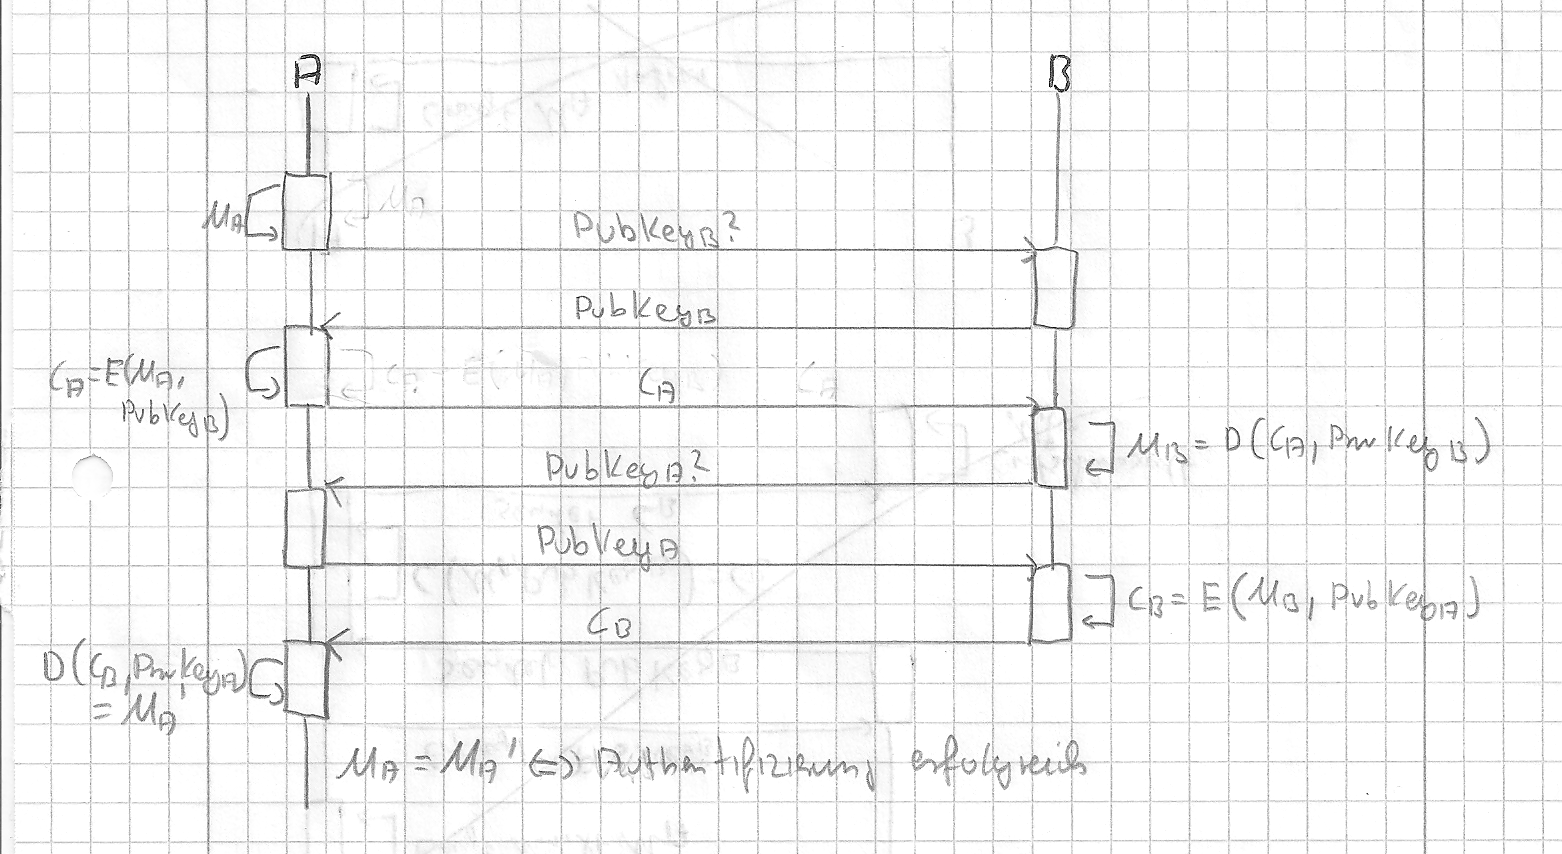
\includegraphics[width=\textwidth]{authentifizierung.png}
  \caption{Gegenseitige Authentifizierung mit RSA}
  \label{fig:authentifizierung}
\end{figure}

\begin{figure}[h]
  \centering
  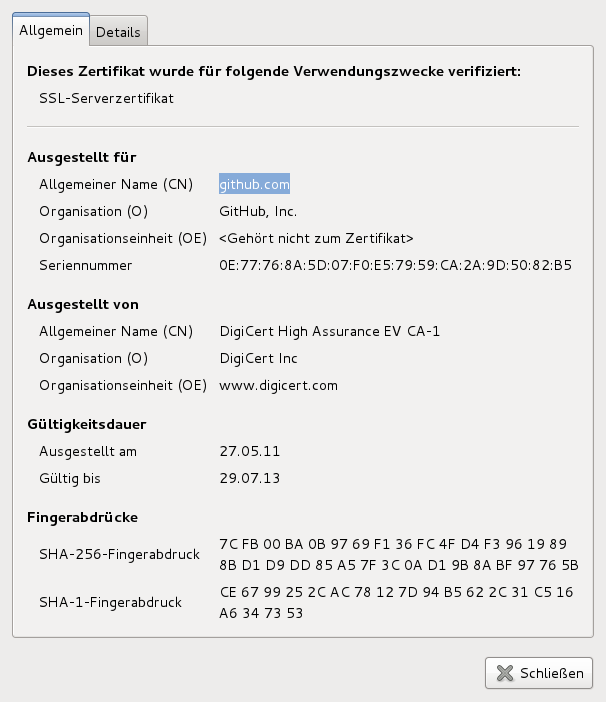
\includegraphics[scale=.5]{github.png}
  \caption{Zertifikat von github.com}
  \label{fig:zertifikat_github}
\end{figure}

\begin{figure}[h]
  \centering
  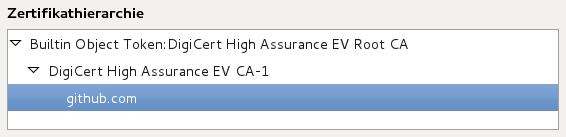
\includegraphics[scale=.5]{hierarchie.png}
  \caption{Zertifikatshierarche des Zertifikats aus
    Abbildung~\ref{fig:zertifikat_github}}
  \label{fig:hierarchie}
\end{figure}

\end{document}
